%%%%%%%%%%%%%%%%%%%%%%%%%%%%%%%%%%%%%%%%%
% a0poster Portrait Poster
% LaTeX Template
% Version 1.0 (22/06/13)
%
% The a0poster class was created by:
% Gerlinde Kettl and Matthias Weiser (tex@kettl.de)
% 
% This template has been downloaded from:
% http://www.LaTeXTemplates.com
%
% License:
% CC BY-NC-SA 3.0 (http://creativecommons.org/licenses/by-nc-sa/3.0/)
%
%%%%%%%%%%%%%%%%%%%%%%%%%%%%%%%%%%%%%%%%%

%----------------------------------------------------------------------------------------
%	PACKAGES AND OTHER DOCUMENT CONFIGURATIONS
%----------------------------------------------------------------------------------------

\documentclass[a1,portrait]{a0poster}
\usepackage{geometry}
 \geometry{
 a1paper,
 left=5cm,
 right=0mm,
 top=5cm,
 bottom=20mm,
 }
\usepackage{multicol} % This is so we can have multiple columns of text side-by-side
\columnsep=50pt % This is the amount of white space between the columns in the poster
\columnseprule=3pt % This is the thickness of the black line between the columns in the poster

\usepackage[svgnames]{xcolor} % Specify colors by their 'svgnames', for a full list of all colors available see here: http://www.latextemplates.com/svgnames-colors

\usepackage{times} % Use the times font
%\usepackage{palatino} % Uncomment to use the Palatino font

\usepackage{graphicx} % Required for including images
\graphicspath{{figures/}} % Location of the graphics files
\usepackage{booktabs} % Top and bottom rules for 
\usepackage[font=small,labelfont=bf]{caption} % Required for specifying captions to tables and figures
\usepackage{amsfonts, amsmath, amsthm, amssymb} % For math fonts, symbols and environments
\usepackage{wrapfig} % Allows wrapping text around tables and figures
\usepackage{hyperref} % for \url command

\begin{document}

%----------------------------------------------------------------------------------------
%	POSTER HEADER 
%----------------------------------------------------------------------------------------

% The header is divided into two boxes:
% The first is 75% wide and houses the title, subtitle, names, university/organization and contact information
% The second is 25% wide and houses a logo for your university/organization or a photo of you
% The widths of these boxes can be easily edited to accommodate your content as you see fit

\begin{minipage}[b]{0.75\textwidth}
\Huge \color{NavyBlue} \textbf{Analysing Student Performance During Tests} \color{Black}\\ % Title
\huge\textit{By Analysing the History of the Code}\\[2cm] % Subtitle
\Large \textbf{Kurt McAlpine}\\[0.5cm] % Author(s)
\Large University of Auckland\\[0.4cm] % University/organization
\large \texttt{kmca733@aucklanduni.ac.nz}\\
\end{minipage}
%
\begin{minipage}[b]{0.25\textwidth}

\includegraphics[width=10cm]{logo.png}\\
\end{minipage}

\vspace{1cm} % A bit of extra whitespace between the header and poster content

%----------------------------------------------------------------------------------------

\begin{multicols}{2} % This is how many columns your poster will be broken into, a portrait poster is generally split into 2 columns

%----------------------------------------------------------------------------------------
%	ABSTRACT
%----------------------------------------------------------------------------------------

\color{Navy} % Navy color for the abstract

\begin{abstract}

Software engineering courses today have impractical test environments. They are
performed using pen and paper, without access to a computer, compiler, IDE or
the internet. Active Test Programmer gives the students the opportunity to be
tested in a practical manner and gives the teacher confidence that plagiarism
will be caught. Practical tests will give students a more realistic assessment
of their abilities in the real world. Practical tests also give industry
recruiters more confidence that students that graduate from such programmes have
good practical skills. 

\end{abstract}

%----------------------------------------------------------------------------------------
%	INTRODUCTION
%----------------------------------------------------------------------------------------

\color{SaddleBrown} % SaddleBrown color for the introduction

\section*{Introduction}

In the world today, programming and programs are prevalent and abundant in our
every day lives. Therefore it is an important skill. It's
widely accepted that programming is a difficult skill to learn
\cite{jenkins2002difficulty, robins2003learning}. There is a need to innovate
and devise solutions to help students be more effective in class.
When students struggle in class with tests and assignments, it can lead to
plagiarism or even dropping out\cite{bennedsen2007failure}. Currently in many
institutions, software engineering courses test their students on their
knowledge and skill in a way that is artificial to real world programming.
For example, tests are done with pen and paper and without access to computers with
IDE`s, compilers or the internet. Therefore, in this project we want to construct a
way to give software engineering students robust testing environments that allow
students to have a more realistic set of tools during the test. However, whilst
giving students these tools we would also like to give the teaching staff
confidence that plagiarism can be detected automatically without tedious manual
inspection of student submissions as well as detecting plagiarised work that the
student has attempted to conceal.

%----------------------------------------------------------------------------------------
%	OBJECTIVES
%----------------------------------------------------------------------------------------

\color{DarkSlateGray} % DarkSlateGray color for the rest of the content

\section*{Description of Tools}

We have implemented a plugin for the Eclipse IDE that allows students to take a
programming test in class using their own laptop or this plugin can be
installed in laborartory computers. The plugin allows students to take a
programming test with fully featured IDE. While the student is taking the test
the Eclipse plugin records the changes to the files, once every second a diff
of the file is stored in a git repository. When the student has finished the
test they submit their Eclipse workspace.

\begin{center}\vspace{1cm}
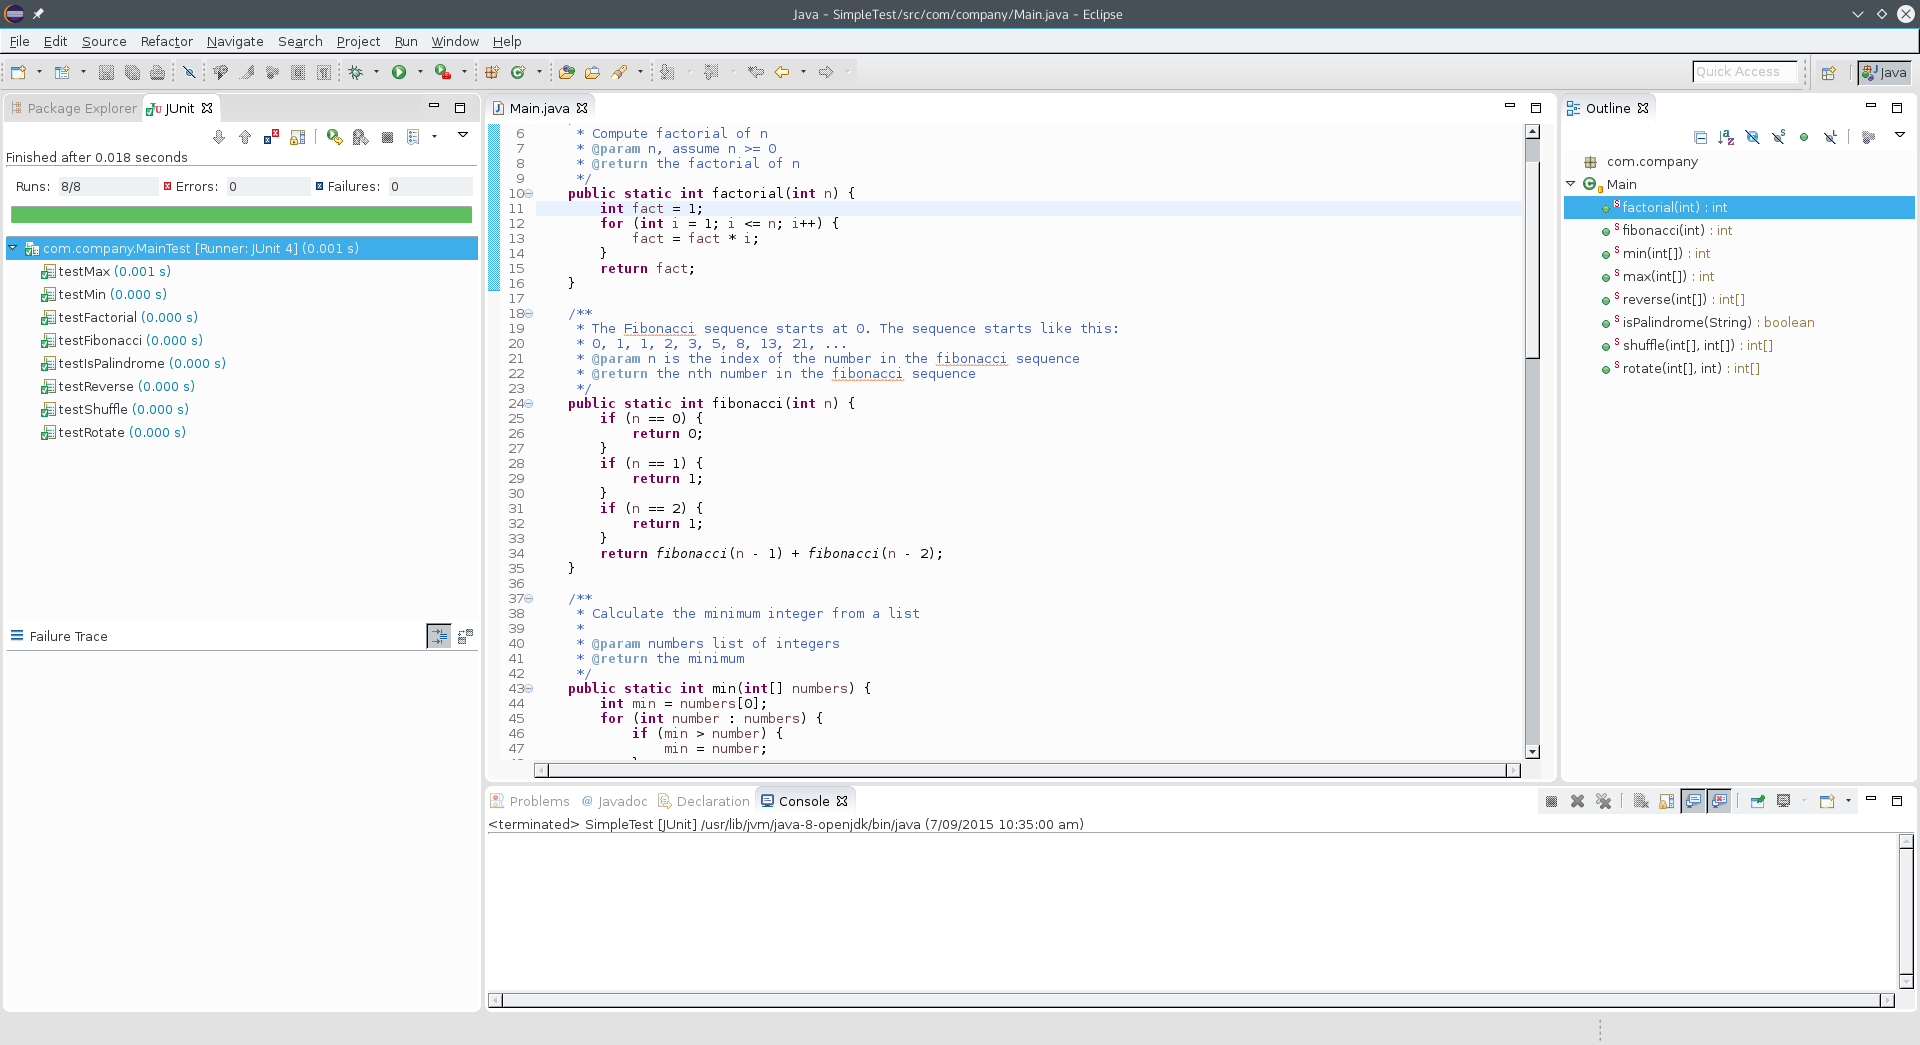
\includegraphics[width=0.8\linewidth]{eclipse}
\captionof{figure}{\color{Green} Screenshot of a test in progress}
\end{center}\vspace{1cm}

Once all student submission have been collected we can begin the analysis of
the tests. Using a command line application that we have implemented
(\url{https://github.com/kurtmc/CodeReportTool}) we can begin to analyse the
student tests.

Some of the basic analytics we can get out of the tool are:
\begin{itemize}
	\item Time taken to complete test
	\item Average characters typed per minute
\end{itemize}

A more advanced analysis that is performed is to calculate the time the student
has spent modifying and adding code in particular nodes in the abstract syntax
tree. For example, it may be relevant for the teacher of a class to see where
students struggle the most. The programming test may consist of several
functions that need to be implemented each function relevant to a certain
topic. It may be useful for the intructor to know how long it takes students to
complete these functions and therefore determine if he or she needs to spend
for time in class going over the topic related to the functions that took
students the longest to implement.


 %----------------------------------------------------------------------------------------
%	REFERENCES
%----------------------------------------------------------------------------------------

{\small
\nocite{*} % Print all references regardless of whether they were cited in the poster or not
\bibliographystyle{plain} % Plain referencing style
\bibliography{references} % Use the example bibliography file sample.bib
}

%----------------------------------------------------------------------------------------
%	ACKNOWLEDGEMENTS
%----------------------------------------------------------------------------------------

\section*{Acknowledgements}

Etiam fermentum, arcu ut gravida fringilla, dolor arcu laoreet justo, ut imperdiet urna arcu a arcu. Donec nec ante a dui tempus consectetur. Cras nisi turpis, dapibus sit amet mattis sed, laoreet.

%----------------------------------------------------------------------------------------

\end{multicols}
\end{document}
